\section{Results and Discussion}\label{sec:Discussion}
\subsection{Validating the Model}

\begin{table}[ht]
  \begin{tabular}{r|rr}
    \toprule
    N   & Numerical & Analytical \\
    1   & \(1.5\pm 0.0\)          &   1.5        \\
    2   &  \(3.0 \pm 0.0\)         &    3       \\
    10  & \(15.0\pm 0.0\)          &    15       \\
    100 &  \(150.0\pm 0.0\)         &   150        \\
    \bottomrule
  \end{tabular}
  \caption{Expected local energy for non-interactive particles in 3D spherical potential compared to analytical
    solution for \(\alpha = 0.5\) for different number of particles. By~\eqref{eq:noninteracting}, there is no
    spatial dependency, making the comparison easy. The numerical results agree
    perfectly with the analytical value.}
  \label{tab:1}
\end{table}

To validate that our implementation is working correctly, the model is run for a
spherical potential without any interactions. The expected local energy is
compared to the analytical solution, summarized in~\vref{tab:1}. The
computed energies are exactly \(\frac{d}{2}\) of the number of particles, as
expected from~\vref{eq:noninteracting}.

\begin{figure}[ht]
  \centering
  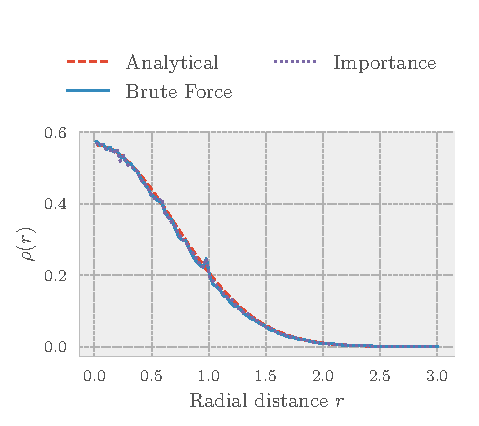
\includegraphics[]{figures/density1.pdf}
  \caption{One-body density of 1 boson in 1 dimension, using $N = \num{1e6}$ cycles, $\omega = 1$, $\alpha = 0.5$.}
  \label{fig:1 part 1 dim density}
\end{figure}

\begin{figure}[ht]
  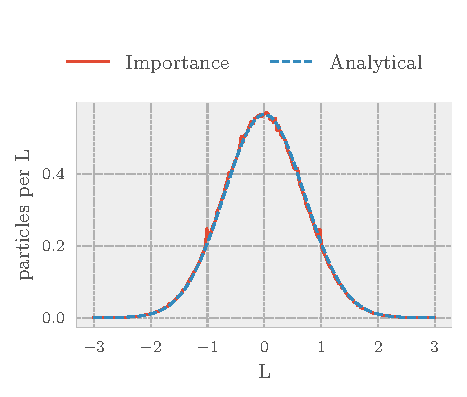
\includegraphics[]{figures/density2.pdf}
  \caption{Radial one-body density of 2 non-interacting bosons in 3 dimensions, using $N = \num{1e6}$ cycles, $\omega = 1$, $\alpha = 0.5$.}
  \label{fig:2 part 3 dim density}
\end{figure}


Further validation is performed by comparing the one body density found from
brute force sampling, importance sampling and analytical solution~\cref{eq:driftforce}
shown in~\vref{fig:1 part 1 dim density}. Aside from the statistical noise
introduced by the finite number of Monte-Carlo cycles, the approximated
densities follow the analytical result closely. \Cref{fig:2 part 3 dim
  density} demonstrates how this scales with more particles and dimensions,
as seen from the radial onebody density of two particles in three dimensions.

\subsection{Blocking of Local Energy}
\begin{figure}
  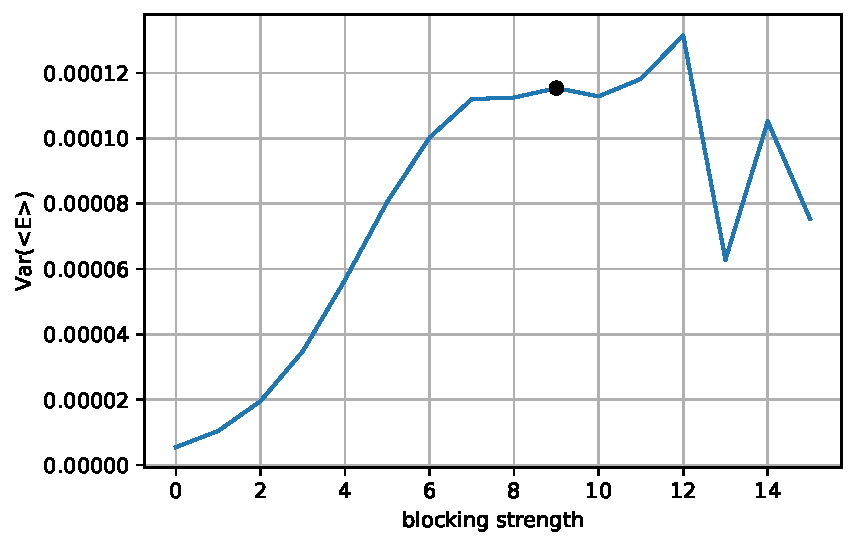
\includegraphics{figures/blocking1.pdf}
	\centering
	\caption{Variance of the estimate of $\langle E_{L} \rangle$ using blocked values of local
      energy at various strengths. As the blocking strength increases, the
      autocorrelation is decreased and variance increases before it plateaus,
      shown with the black dot. The data have been produced for 40
      non-interacting bosons in three dimensions using $N = 2^{20}$ cycles, $\alpha =
      0.8$, $\omega = 1$, with and without importance sampling}
	\label{fig:blocking1}
\end{figure}

The effect of applying blocking on the local energy before calculating the
variance is shown in~\cref{fig:blocking1}. Although the local energies are
sampled from an approximately correct distribution, the data is produced by moving a single
boson at a time. The move may be rejected by the metropolis
algorithm, causing no change in state. Because of this, the data is highly correlated,
leading to an underestimation of the variance as seen for the unblocked data.
The variance stabilizes after repeated blocking, when the data is
approximately uncorrelated. Note that this happens at different strength
for brute force sampling and importance sampling. From~\cref{fig:blocking1}
the latter requires a weaker blocking strength, indicating that
the data created are less correlated. This is expected as
importance sampling uses additional information from the wave function and
explores the space of states more efficiently than brute force.
The variance stabilizes at strength $6$ when
using importance sampling as opposed to $9$ when using brute force, granting
eight times the effective amount of data and thus a smaller variance of the
estimator.


\begin{figure}[ht]
	\centering
	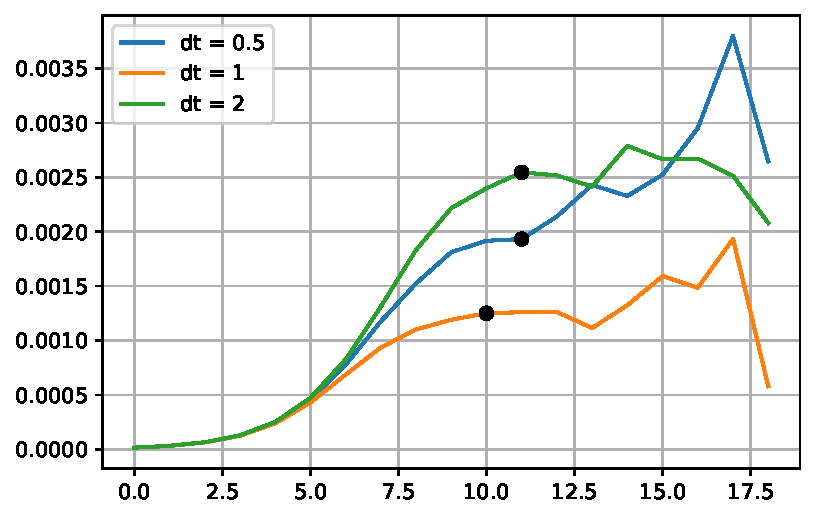
\includegraphics[]{figures/blocking3.pdf}
	\caption{Variance of the estimate of $\langle E\rangle$ using blocked values
      of local energy at various strengths. The data has been produced for 40
      non-interacting bosons in 3 dimensions, using $N = 2^{20}$ cycles, $\alpha =
      0.8$, $\omega = 1$, using importance sampling with step length $0.5$, $1$
      and $2$, respectively} 
	\label{fig:blocking2}
\end{figure}

\begin{table}[t]
	\begin{tabular}{lclclclc}
		\hline
		\hline
      dt & \(\langle E \rangle \)& blocking strength\\
		\hline
		0.5 & \(68.009 \pm 0.044\) & 11\\
		1 & \(68.039 \pm 0.035\) & 10\\
		2 & \(67.942 \pm 0.050\) & 11\\
		\hline
	\end{tabular}
	\caption{Estimate of energy $\langle E \rangle$ for 40 particles, $\alpha = 0.3$, $\omega = 1$}
	\label{tab:blocking}
\end{table}

The effect of blocking for a larger system is shown in
\cref{fig:blocking2} using only importance sampling and step lengths of
$0.5$, $1$ and $2$. As only a single particle is moved in each MC cycle,
increasing the size of the system results in a comparatively smaller change.
The local energies will invariably become more correlated, which is apparent
when comparing the blocking strengths from~\cref{fig:blocking2} to~\cref{fig:blocking1}.

Further, the least correlated data was produced with a step length of $\delta t = 1$,
requiring blocking strength $10$ as opposed to $11$ for $\delta t = 0.5$ and
$2$. Using a step length too small results in the local energy changing
minimally from cycle to cycle, increasing the correlation and minimizing the
effective amount of data. The same happens if the step length is too big, as
large moves will tend to be rejected often, causing repeated values to be
sampled. \autoref{tab:blocking} presents the resulting estimates of energy with
the uncertainty established using the blocking. The estimated
energy is only sensitive to the step length in the sense that more cycles may be
needed to get an accurate result of the step length is taken too small or too
big.

 
\subsection{Energy of Non-Interacting System}
\begin{figure}[ht]
  \centering
  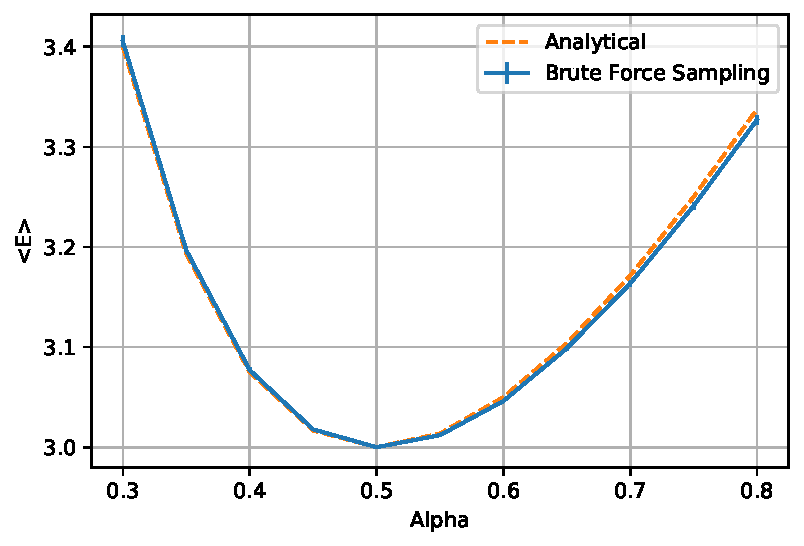
\includegraphics[]{figures/energy_importance1.pdf}
  \caption{\label{fig:energybyalpha} The expected local energy as function of
    the variational parameter \(\alpha\) for both brute force and importance
    sampling, compared to the analytical solution. The system consists of two
    non-interacting bosons using \(2^{17}\) cycles.}
\end{figure}
\begin{figure}[ht]
  \centering
  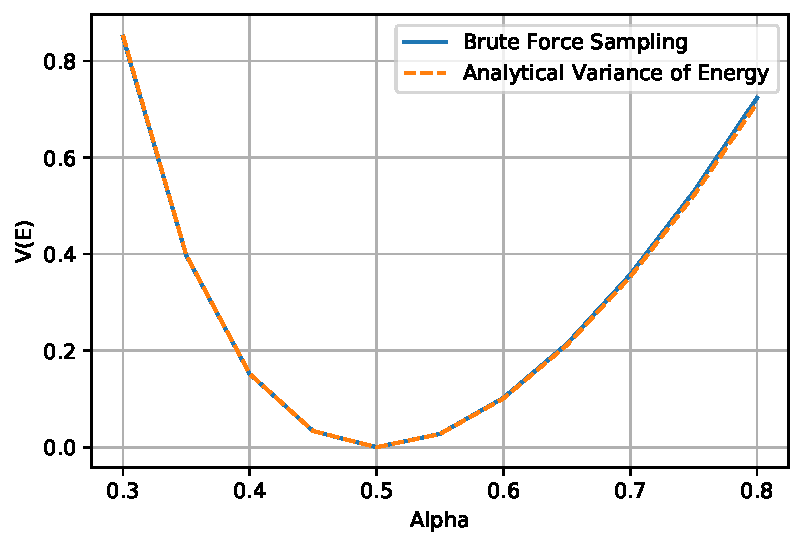
\includegraphics[]{figures/variance_importance1.pdf}
  \caption{\label{fig:variancebyalpha} The variance of the expected local energy as function of
    the variational parameter \(\alpha\) for both brute force and importance
    sampling, compared to the analytical solution. The system consists of two
    non-interacting bosons using \(2^{17}\) cycles.}
\end{figure}

Varying the variational parameter \(\alpha\) gives different trial wave
functions that have different expected local energy. For the non-interacting
spherical system there are analytical solutions for the \(\alpha\)-dependency of
the
local energy, and can be used to validate our model. This comparison is shown
in~\cref{fig:energybyalpha} and~\cref{fig:variancebyalpha}. The curves overlap
within the MC-uncertainty as expected, with the minimum occurring at
\(\alpha=0.5\), giving confidence in the implementation.

\subsection{Numerical and Analytical Laplacian}
\begin{figure}[ht]
	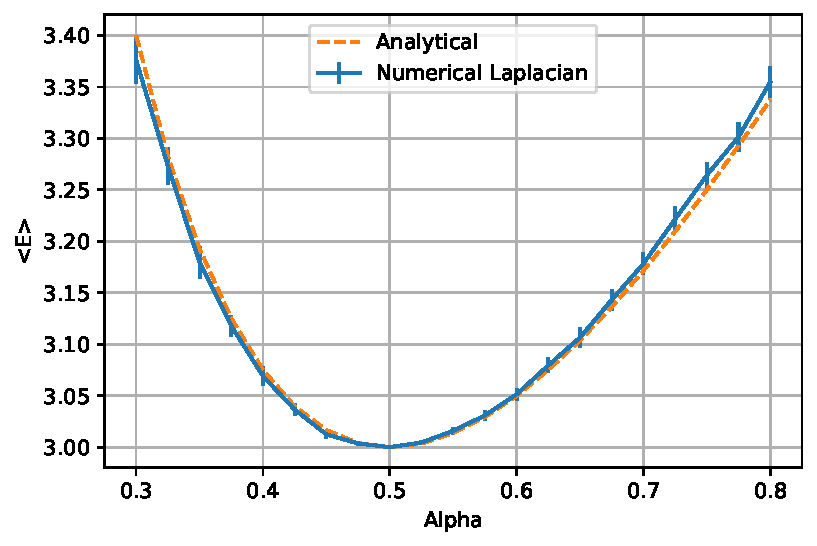
\includegraphics[]{figures/numericalLap.pdf}
	\centering
	\caption{Estimated energy $\langle E_{L} \rangle$ for two non-interacting
      bosons, comparing the analytical solution to numerically evaluated
      Laplacian. $2^{17}$ cycles, $\omega = 1$ and importance sampling was used. Errorbars was established using blocking. }
	\label{fig:numerical lap}
\end{figure}

\begin{figure}[ht]
	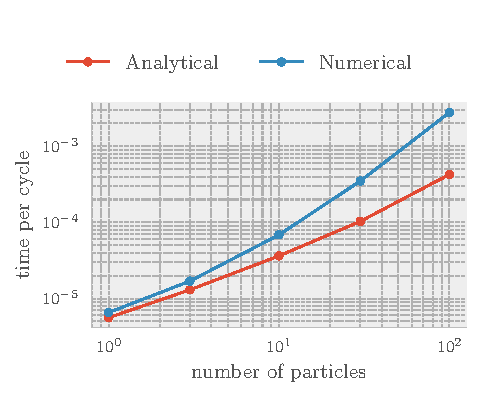
\includegraphics[]{figures/numericalTime.pdf}
	\centering
	\caption{Comparison of CPU-time of numerical and analytical Laplacian for
      different numbers of particles. The timing is with respect to the whole
      simulation. However, as the uninteresting steps
    are of \(\mathcal{O}(1)\), they irrelevant when comparing the graphs.}
	\label{fig:numerical time}
\end{figure}

When evaluating the Hamiltonian, one can choose to use the analytical expression
for the Laplacian or compute it numerically using finite differences. Both
methods give the same solution, as illustrated by~\cref{fig:numerical lap}.
Suspecting that the computational cost differs, their CPU time are plotted
in~\cref{fig:numerical time}. The difference is negligible with few particles,
but the numerical Laplacian quickly outgrows the analytical, showing exponential
dependency on the number of particles. Most potentials do now have analytical
solution, having to rely on the much slower numerical computation. 

\subsection{Interacting Potentials}
\begin{figure}[ht]
	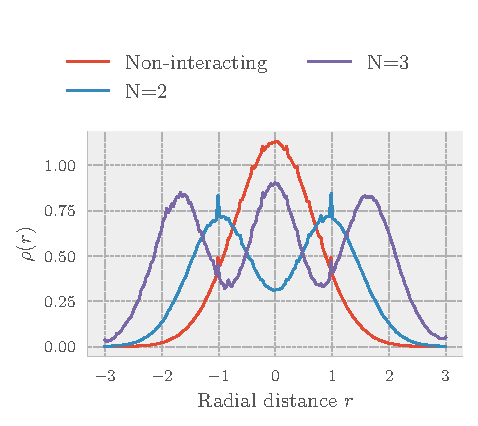
\includegraphics[]{figures/interactingDensity.pdf}
	\centering
	\caption{One body density \(\rho\) in one dimension for two non-interacting
      bosons, two interacting bosons, and three interacting bosons.
      Non-interacting bosons occupies the same space to minimize the energy,
      while the interacting bosons separate. The more bosons, the more they
      spread out.}
	\label{fig:interacting density}
\end{figure}

Adding interaction between the bosons drastically changes the behavior of the
system. In~\cref{fig:interacting density} non-interacting bosons are compared to
systems having two and three interacting bosons. The densities of the latter are
spread out, with maxima directly proportional to the number of particles. The
interpretation is that the interacting particles are repelled by each other and
attempts to minimize their energy while staying within the potential, resulting
in \(N\) bumps becoming more and more spread out as \(N\) grows.


\subsection{Optimal Parameter \(\alpha\)}
\begin{figure}[ht]
	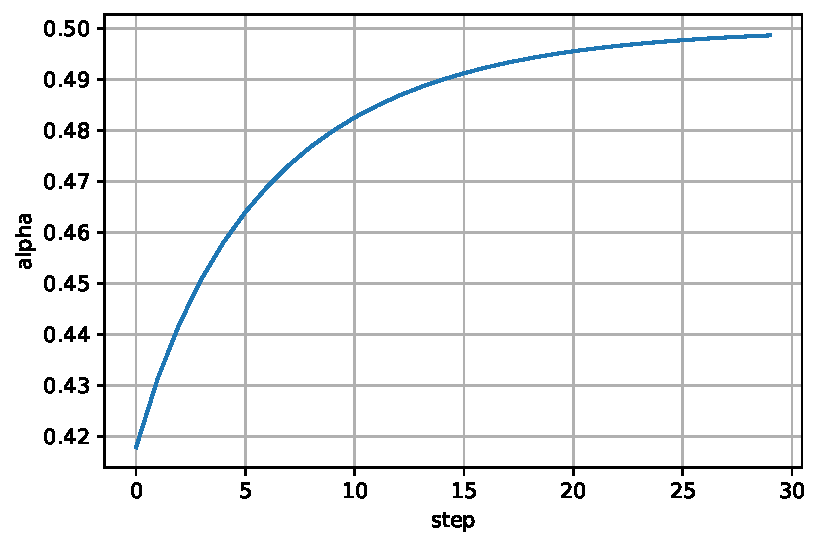
\includegraphics[]{figures/gd.pdf}
	\centering
	\caption{Gradient decent on the parameter $\alpha$ for two non-interacting
      bosons with different \(\alpha_{0}\), learning rate $\mu = 0.01$, $N = 10000$ steps and $\omega = 1$}
	\label{fig:gd}
\end{figure}

Gradient descent was performed on the variational parameter \(\alpha\) with
non-interactive bosons. \Cref{fig:gd} shows the results. The method is robust
for different initial guesses \(\alpha_{0}\), all converging to \(0.5\) as
expected. This establishes confidence that the method will converge to the
optimal \(\alpha\) in the interacting case where the analytical solution is not known.

\subsection{Interacting Bosons in Elliptical Potential}

\begin{table}[t]
	\begin{tabular}{lclclclc}
		\hline
		\hline
		Bosons & \(\langle E \rangle\) & optimal $\alpha$\\
		\hline
		10 & \(24.3985 \pm 0.0011\) & 0.49752\\
		50 & \(127.37 \pm 0.035\) & 0.48903\\
		100 & \(265.69 \pm 0.27\) & 0.48160\\
		\hline
	\end{tabular}
	\caption{Estimate of energy $\langle E \rangle$ for 10, 50 and 100 particles in elliptical potential. $\beta = \gamma = 2.8284$. $N = 2^20$ cycles per thread, of $12$ threads. Importance sampling with a step length $0.5$ was used. Gradient decent was used to optimize $\alpha$}
	\label{tab:energies}
\end{table}

\begin{figure}
	\begin{subfigure}{\textwidth}
		\centering
		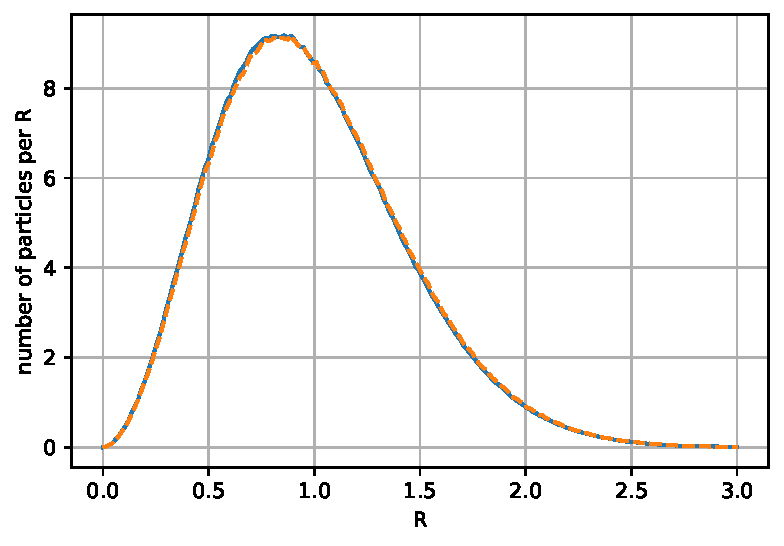
\includegraphics[width=.8\linewidth]{figures/density10.pdf}
		\subcaption{Radial onebody density for $10$ bosons in elliptical trap, interacting and non-interacting case}
	\end{subfigure}%
	\begin{subfigure}{\textwidth}
		\centering
		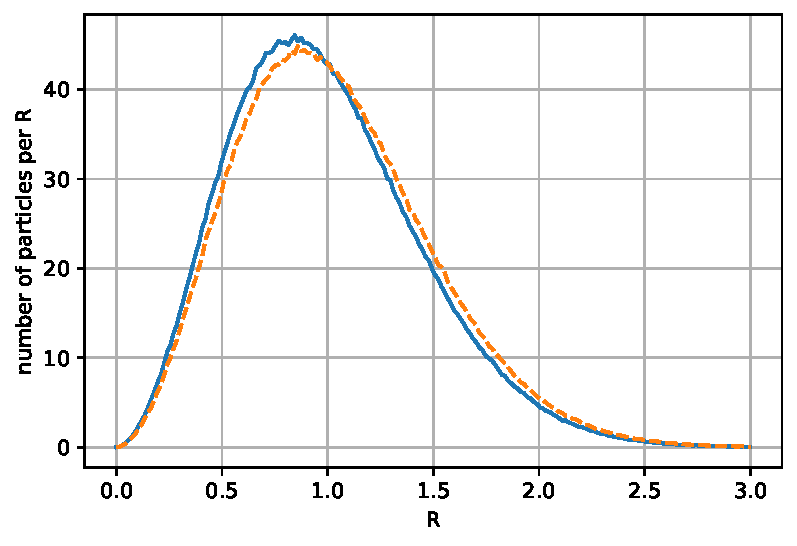
\includegraphics[width=.8\linewidth]{figures/density50.pdf}
		\subcaption{Radial onebody density for $50$ bosons in elliptical trap, interacting and non-interacting case}
	\end{subfigure}%
	\begin{subfigure}{\textwidth}
		\centering
		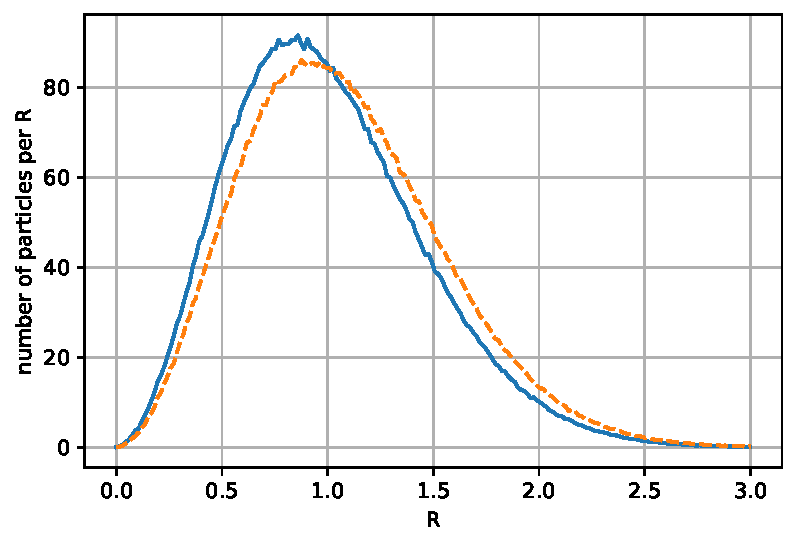
\includegraphics[width=.8\linewidth]{figures/density100.pdf}
		\subcaption{Radial onebody density for $100$ bosons in elliptical trap, interacting and non-interacting case}
	\end{subfigure}%
	\centering
	\caption{Comparison of the radial onebody density for interacting and non-interacting bosons. The hardshell radius of in the interacting case is $a = 0.0043$. The elliptical potential is defined by $\beta = \gamma =  2.82843$. }
	\label{fig:ellipticalOnebodyDensity}
\end{figure}

\autoref{tab:energies} presents the estimated ground state energies for $10$,
$50$ and $100$ interacting bosons confined by a elliptical potential. The
optimal value for $\alpha$ was found using gradient decent. Notice that the
optimal value is decreasing with the number of particles in the interacting
case, whereas it is analytically $\alpha = 0.5$ in the non-interacting case for
any number of particles. A smaller value of $\alpha$ indicates the onebody
exponential functions widens, resulting in a wider distribution of particles.
This makes sense, as hardshell bosons interact repulsively. Therefore, the more
particles, the more energetically favorable it is to spread out. This is
consistent with the 1D result presented in
\autoref{fig:ellipticalOnebodyDensity}. As the number of particles increase, the
radial onebody density tends to migrate outward with respect to the
non-interacting system.


The ground state energy was most accurately calculated for $10$ bosons. This is
because, as discussed earlier, data tend to be less correlated for smaller
systems. To get an accurate estimate for larger systems, a increase in the number
of cycles is appropriate. Due to the increasing CPU-demand, a trade-off must be
made between time and accuracy.


A comment on the interpretation of the error presented in \autoref{tab:energies} is appropriate:
The error is an estimate of the statistical error in the estimated ground state
energy introduced by the Monte-Carlo simulation. It does not account for
possible error introduced in the estimation of $\alpha$ that minimizes the
energy. This is much harder to quantity, and is possibly large in the case for
$50$ and $100$ particles, as the gradient was hard to estimate consistently.
Furthermore, the error does not in any way establish a confidence interval for
the true ground state value of the Hamiltonian we are investigating, which is
harder still to quantify. Our estimate a approximate minimum only in the
subspace spanned by out trial wave function, which is hopefully, somewhat close
the exact solution of the system.








%%% Local Variables:
%%% mode: latex
%%% TeX-master: "../main"
%%% End:
